\documentclass{utea-tarea}

\newcommand*{\nombre}{Nombres Apellidos}
\newcommand*{\profesor}{lava}
\newcommand*{\codigo}{0020240101}
\newcommand*{\curso}{Física I}
\newcommand*{\tarea}{Vectores y cinemática}
\newcommand*{\fecha}{16/07/2024}

\usepackage{amsmath,amssymb}
\usepackage{tikz}
\usetikzlibrary{babel}

\usepackage{natbib}
\setlength{\parindent}{0pt}

\begin{document}
\maketitle

\section*{Caso 1}
[5p] Con los vectores del diagrama obtenga:

\begin{enumerate}
    \item Obtenga y grafique: $\vec{A} + \vec{B}$
    \item Obtenga y grafique: $\vec{A} - \vec{B}$
\end{enumerate}

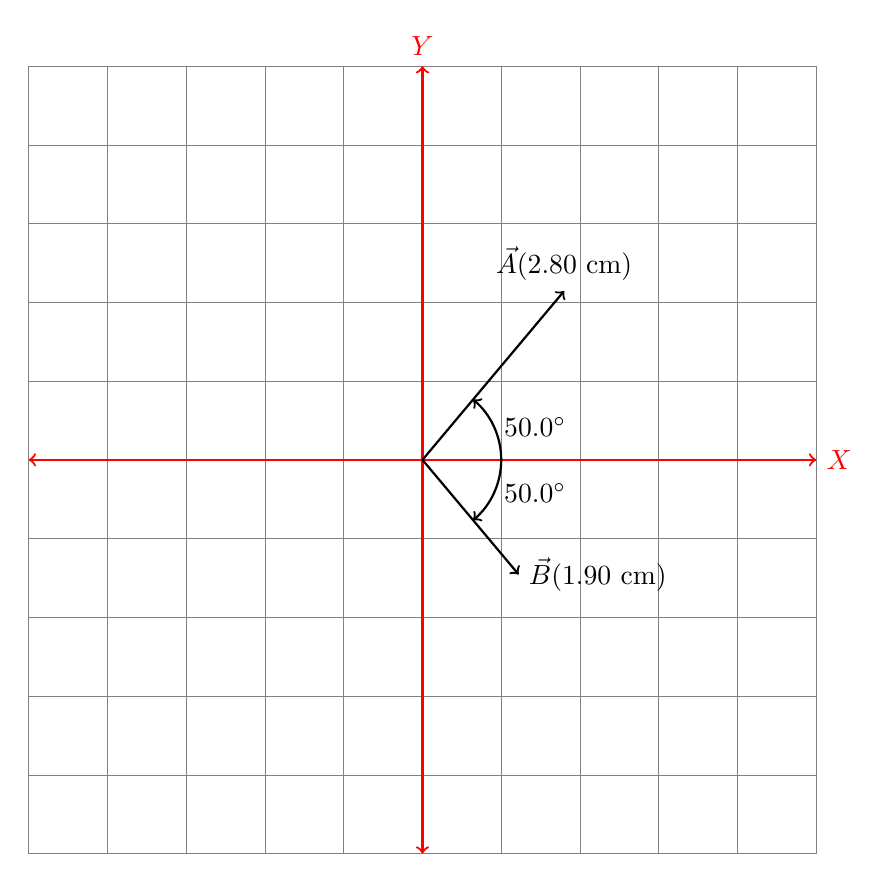
\begin{tikzpicture}[scale=1]
    \draw[help lines,step=1,color=gray] (-5,-5) grid (5,5);
    \draw [<->,thick,red] (-5,0) -- (5,0) node [right] {$X$};
    \draw [<->,thick,red] (0,-5) -- (0,5) node [above] {$Y$};

    \draw [->,thick] (0,0) -- (50:2.8) node [above] {$\vec{A} (2.80 \text{ cm})$};
    \draw [->,thick] (1,0) arc (0:50:1) node [midway,right] {$50.0^\circ$};
	
    \draw [->,thick] (0,0) -- (-50:1.9) node [right] {$\vec{B} (1.90 \text{ cm})$};
    \draw [->,thick] (1,0) arc (0:-50:1) node [midway,right] {$50.0^\circ$};
\end{tikzpicture}


\section*{Caso 2}
[5p] Un automóvil está detenido ante un semáforo. Después, viaja en línea recta y su distancia con respecto al semáforo está dada por $x(t) = bt^2 - ct^3$, donde $b = 2.40 \, m/s^2$ y $c = 0.120 \, m/s^3$.

\begin{enumerate}
    \item Calcule la velocidad media del automóvil entre el intervalo $t = 0$ a $t = 10.0 \, s$.
    \item Calcule la velocidad instantánea del automóvil en $t = 0, t = 5.0 \, s$ y $t = 10.0 \, s$.
    \item  ¿Cuánto tiempo después de que el auto arrancó vuelve a estar detenido? \citep{Young2013}
\end{enumerate}

\paragraph{SOLUCIÓN:}
\begin{enumerate}
    \item \cite{Young2013} define la velocidad media como $\Bar{v} = \dfrac{\Delta x}{\Delta t}$
    $$\Bar{v} = \frac{\Delta x}{\Delta t} = \frac{x(10.0) - x(0)}{10.0 - 0} = \frac{120.0 - 0}{10.0} = 12$$
    \textbf{Rpta:} la velociada media es $12 \, m/s$.
    \item \cite{Young2013} define la velocidad instantánea por $v = \dfrac{dx}{dt}$, entonces $v=2bt - 3ct^2$
    \begin{enumerate}
        \item $v(0) =2b(0) - 3c(0)^2 = 0$, la velocidad en $t=0$ es $0 \, m/s$
        \item $v(5.0) =2b(5.0) - 3c(5.0)^2 = 15.0$, la velocidad en $t=5.0$ es $15.0 \, m/s$
        \item $v(10.0) =2b(10.0) - 3c(10.0)^2 = 12.0$, la velocidad en $t=10.0$ es $12.0 \, m/s$
    \end{enumerate}
    
    \item El auto vuelve a estar detenido cuando $v(t)=0=2bt - 3ct^2=t(2b - 3ct)$, es decir:
    $$\begin{cases}t &= 0 \\ t &= \dfrac{2b}{3c} \end{cases}$$
    \textbf{Rpta:} El auto vuelve a estar detenido después de $13.3 \, s$
\end{enumerate}

\bibliographystyle{apalike2}
\bibliography{referencias}

\end{document}
